\todo{Applicationlayer einführen, die use cases zu den 3 Kategorien sind geschrieben}
\todo{Bilder zu Use Cases einfügen}
\chapter{Application layer und Use Cases\label{chap:usecases}}
\section{Application Layer}
\todo{was über den applayer erzählen}
\begin{figure}[htbp]
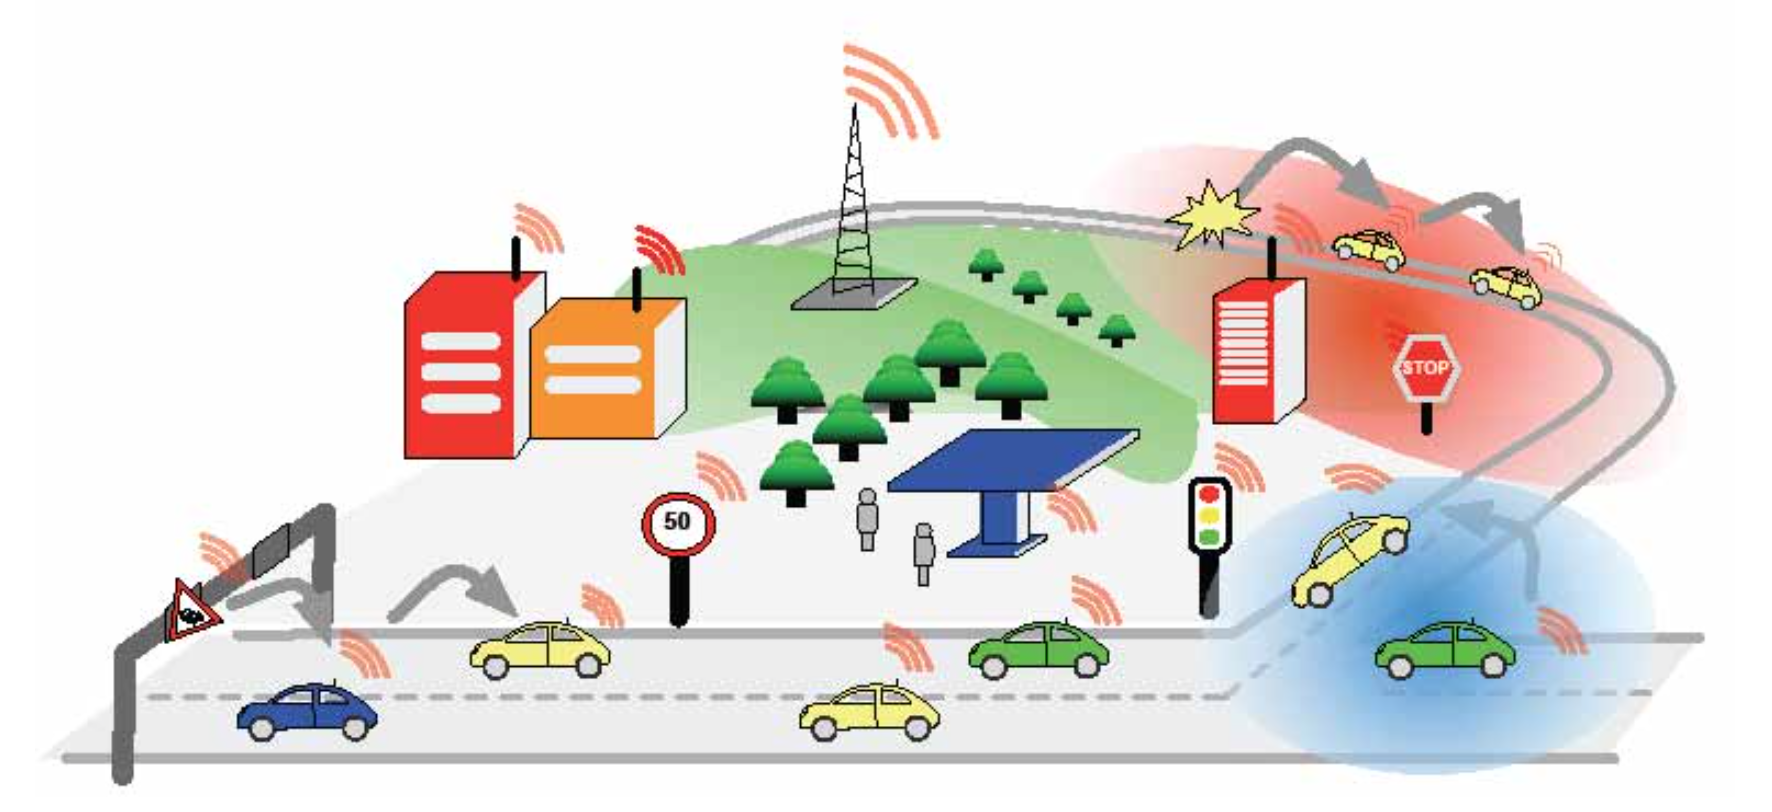
\includegraphics[width=0.99\textwidth]{content/images/06_use_cases/komponenten.png}
\caption{Die Komponenten der \acl{C2C}}
\label{fig:komponentenderc2x}
\end{figure}
Die \acl{C2C} bietet eine große Vielfalt an verschiedenen Einsatzmöglichkeiten. Da es sich bei dem gesamten Projekt nicht nur darum handelt das Fahrzeuge untereinander kommunizieren, sondern wie auf \autoref{fig:komponentenderc2x} zu sehen auch andere Verkehrskomponenten. Um das Zusammenspiel der Komponenten besser zu verstehen und zu sehen wie groß das Potential der \acl{C2C} ist, werden im folgenden mehrere Szenarien aufgezählt und erklärt. 

\section{Use cases}
\subsection{Sicherheitsbedingt}
Sicherheitsbedingte Szenarien sind Fälle bei denen ein Möglicher Unfall verhindert werden kann. Im Folgenden werden drei Szenarien erklärt bei denen das Unfallrisiko minimiert werden kann.

\subsubsection{Cooperative Forward Collision Warning}
Einer der häufigsten Ursachen für Verkehrsunfälle sind plötzliche Bremsmanöver von Vorrausfahrenden Fahrzeugen und die Unaufmerksamkeit eines Fahrers. Aus diesen Ursachen besteht ein erhöhtes Risiko für Auffahrunfälle. Cooperative Forward Collision Warning versucht genau dieses Risiko zu vermindern. Um dies zu vollbringen überwacht jedes Fahrzeug die eigenen Informationen, wie die Geschwindigkeit, Richtung und Position und vergleicht diese mit den Daten der anderen Fahrzeugen. Bei Auffälligkeiten und Abweichungen warnt das System dem Fahrer frühzeitig vor einer möglichen Kollision. Diese Warnung kann durch auditive, visuelle oder haptische Alarme signalisiert werden. Da es durchaus sein kann das noch Fahrzeuge, die nicht in dem C2C Netz kommunizieren, unterwegs sind, können über Objekterkennungssensoren diese ebenfalls identifiziert werden. Dadurch sinkt das Risiko noch einmals für die C2C Teilnehmer. Die Informationen werden innerhalb von 20 bis 200 meter geteilt womit auch genug Zeit bleibt um diese Auszuwerten und den Fahrer frühzeitig zu Informieren. \\
Nachfolgend wird gezeigt wie die Use Cases im Standart definiert werden. Dazu solle dieses Beispiel noch einmal dienen.

\textbf{Application name:} Co-operative collision avoidance or mitigation.
\texbf{Short description:} This use case is based on co-operation between vehicles which detect a risk of forward collision.
Such co-operation is achieved to avoid accident either through driver assistance of direct action on the cars.
\textbf{Usage:} Avoid longitudinal collision.
\textbf{Communication mode:} V2X co-operative awareness associated to unicast.
\begin{figure}[htbp]
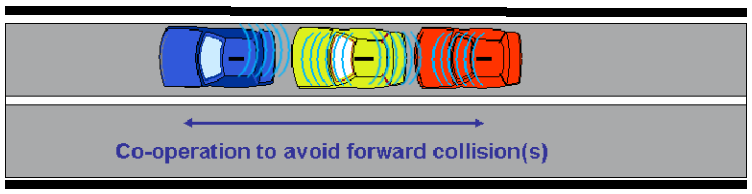
\includegraphics[width=0.99\textwidth]{content/images/06_use_cases/colissionwarning.png}
\caption{Cooperative Forward Collision Warning Use Case}
\label{fig:cfcw}
\end{figure}
\textbf{Main requirements}
\begin{itemize}
\item Capability for a vehicle to broadcast V2X co-operative awareness messages.
\item Capability for this vehicle to establish unicast Peer to Peer sessions to co-operate with other vehicles closely
\item Maximum latency time: 100 ms.
\item Minimum frequency of V2V co-operation awareness messages: 10 Hz.
\item Authenticity of V2X co-operative awareness messages.
\item Vehicles relative positioning accuracy: < 1 m.
following the same path to reduce the risk of accident.
\end{itemize}

\subsubsection{Pre-Crash Sensing/Warning}
Natürlich können nicht alle Unfälle durch die Cooperative Forward Collision Warning vermieden werden. Daher ist davon auszugehen das dennoch Auffahrunfälle geschehen werden. Dafür hat man sich das Pre-Crash Sensing/Warning Szenario ausgedacht, bei dem man von einem Unvermeidbaren Unfall ausgeht. Dies soll durch die \acl{C2C} erkannt und Vorbereitungen für den Unfall getroffen werden. Damit dieses System funktioniert muss wie bei dem vorherigen Szenario dauerhaft Informationen der Fahrzeuge ausgetauscht werden. Dabei geht man davon aus das die Informationen der Fahrzeuge die sich im Umkreis von 20 bis 100 meter befinden überwacht werden müssen. Entdeckt das System einen unvermeidbaren Unfall muss sichergestellt sein das diese Fahrzeuge die Kollidieren werden sicher miteinander kommunizieren können um Daten wie die, Fahrzeuggröße und genaue Position bekannt zu geben. Über diese Informationen können dann Sicherheitsmaßnahmen wie Airbar, Gurtstraffer oder erweiterbare Stoßstangen gesteuert werden und effektiv genutzt werden. 
\begin{figure}[htbp]
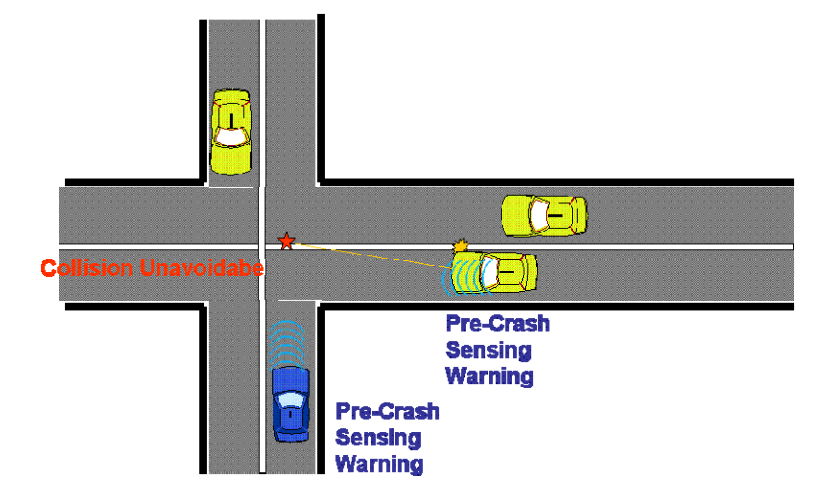
\includegraphics[width=0.99\textwidth]{content/images/06_use_cases/pre_crash_sensing.png}
\caption{Pre-Crash Sensing/Warning Use Case}
\label{fig:pcs}
\end{figure}

\subsubsection{Hazardous Location C2C Notification}
Die Hazardous Location C2C Notification soll dafür sorgen das gefährliche Fahrpassagen weitergegeben werden. Das heisst das System warnt nachkommende Fahrzeuge vor glatten Straßen oder Schlaglöchern. Die Schwierigkeit hierbei ist die Gewinnung der Informationen. Als Beispiel wird genannt das ein Fahrzeug das auf einer glatten Straße fährt und das ESP einsetzt, speichert an welcher stelle, Geschwindigkeit etc. eingetreten ist und diese Nachricht dann weiter sendet. Fahrzeuge die diese Warnnachricht erhalten können dann auf den Umstand mit Verbesserung der Sicherheitsmaßnahmen reagieren oder zumindest dem Fahrer darüber Informieren. 
\begin{figure}[htbp]
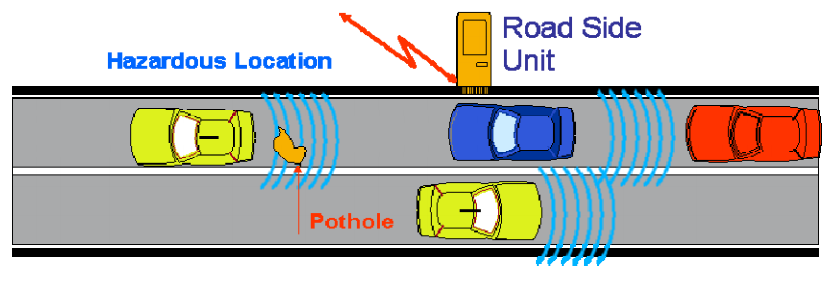
\includegraphics[width=0.99\textwidth]{content/images/06_use_cases/hln.png}
\caption{Hazardous Location C2C Notification Use Case}
\label{fig:hln}
\end{figure}

\subsection{Verkehrseffizienz}
Die Effizienz zu des Verkehrs zu steuern ist der ursprüngliche Sinn der \acl{C2C}. Durch die bessere Leitung des Verkehrs entstehen weniger Staus auf den Straßen, was zu verminderten Stresssituationen für Fahrer führt. Dadurch entstehen verkürzte Wartezeiten für die Teilnehmer am Verkehr und geringere Wartungskosten für die Straßen. Ausserdem kann dadurch die Umwelt mehr geschont werden und die Energiekosten sinken. 

\subsubsection{Enhanced Route Guidance and Navigation}
Navigation ist ein großes Thema das bereits über Navigationssysteme stark verbessert wurde. Enhanced Route Guidance and Navigation soll die Navigation noch einmal verbessern. Dies soll erreicht werden in dem die Fahrdaten von den Roadside Stations gesammelt und ausgewertet werden. Dadurch können Verkehrsaufkommnisse vorhergesagt werden und Fahrzeuge auf ihrem Weg an einer solche Station vorbeikommen können über die aktuellen Verkehrsinformationen aufgeklärt werden und den effektivsten Weg berrechnen um die Verkehrsdichte zu verbessern. Damit dieses Szenario funktioniert müssen die Roadside Stations die Möglichkeit besitzen vorbeifahrende Fahrzeuge zu erkennen und zu Informieren. 
\begin{figure}[htbp]
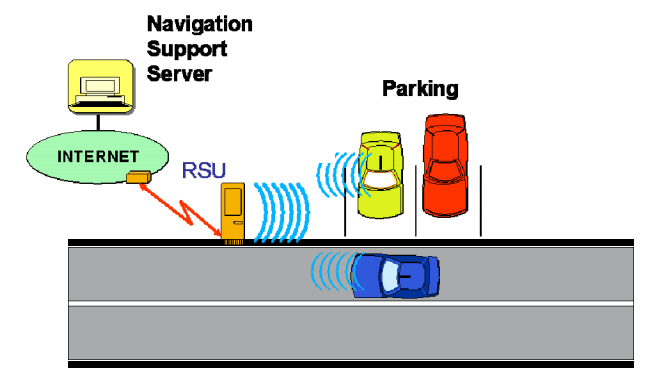
\includegraphics[width=0.99\textwidth]{content/images/06_use_cases/ergn.png}
\caption{Enhanced Route Guidance and Navigation Use Case}
\label{fig:ergn}
\end{figure}

\subsubsection{Green Light Optimal Speed Advisory}
Green Light Optimal Speed Advisory beschäftigt sich mit der optimalen Geschwindigkeit zwischen Ampeln. Damit Fahrzeuge zwischen Ampelabschnitten nicht die Geschwindigkeit reduzieren und nach Möglichkeit nicht immer wieder neu Anfahren müssen, kann durch eine Kreuzung die an der \acl{C2C} teilnimmt Informationen über die Rot-Grün Schaltzeit eingeholt werden. Über den bekannten Abstand zum vorherfahrenden Auto kann die optimale Geschwindigkeit berechnet werden, die das Fahrzeug sich vorwärts bewegen sollte um während einer Grünphase der Ampel dort einzutreffen. Dadurch wird der Verkehrsfluss verbessert und schont die Tankfüllung eines Autos.
\begin{figure}[htbp]
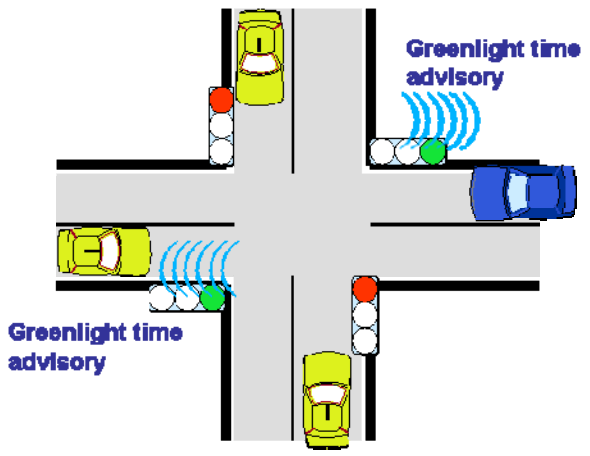
\includegraphics[width=0.99\textwidth]{content/images/06_use_cases/greenlight_opimalspeed.png}
\caption{Green Light Optimal Speed Advisory Use Case}
\label{fig:glos}
\end{figure}

\subsubsection{C2C Merging Assistance}
Bei einfahren in den Verkehr von kann es vorkommen das ein Fahrzeug den fliesenden Verkehr stört. Dadurch entstehen nicht selten Rückstaus die im schlimmsten Fall zu Auffahrunfällen führen. Dies soll über C2C Merging Assistance bereits beim einfahren in den fliesenden Verkehr verhindert werden, in dem das Fahrzeug das in den Verkehr einfliesen möchte die betroffenen Fahrzeuge darüber informiert. Die Fahrzeuge die betroffen sind sollen ihre ihre Geschwindigkeit automatisch reduzieren oder zumindest sollen die Fahrer darüber Informiert werden wie sie sich am besten Verhalten sollen. Dadurch kann der Verkehr weiter sauber fliesen ohne das es im Nachhinein zu einem stillstand kommt. 
\begin{figure}[htbp]
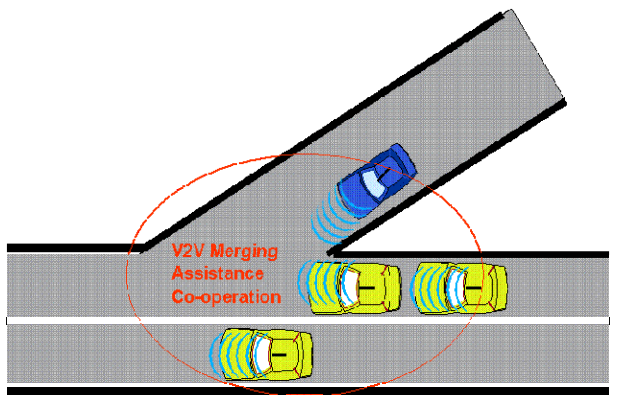
\includegraphics[width=0.99\textwidth]{content/images/06_use_cases/merging_assistance.png}
\caption{C2C Merging Assistance Use Case}
\label{fig:mergingassistance}
\end{figure}

\subsection{Infotainment und andere}
Hier werden die Anwendungsfälle aufgeführt die nicht zur Sicherheit oder Verkehrseffizienz beitragen aber dennoch über die \acl{C2C} realisiert werden. Dazu gehören allgemeine Informationen, Entertainment oder Fahrzeugdaten wie der Verbrauch reduziert werden kann. 

\subsubsection{Internet Access in Vehicle}
Hierbei wird die im Fahrzeug vorhandene Hardware, die dafür da ist mit den anderen Fahrzeugen und Komponenten der \acl{C2C} zu kommunizieren, dafür genutzt um über die Roadside Station ihren Border Gateway auf das Core Netzwerk zuzugreifen und damit auf sämtliche Dienste des Internets. Das bedeutet das alle IP basierten Dienste in einem Fahrzeug nutzbar sind.  \todo{Hier nochmal in dem manifext nachlesen}

\subsubsection{Point of Interest Notification}
Dieser Anwendungsfall ist besonders für Kommerzielle Werbezwecke interessant. Hier werden durch eine Roadside Station Informationen über für den Fahrer interessante Orte zu den Umliegenden Fahrzeugen gesendet. Die Masse an Informationen kann durch das Fahrzeug gefiltert werden und immer Situationsbedingt die passenden Orte vorgeschlagen werden. Zum Beispiel wenn der Benzinstand des Fahrzeuges niedrig ist können die in der nähe befindlichen Tankstellen mit Öffnungszeiten und preise dem Fahrer vorgeschlagen werden. Dadurch wird die Werbung deutlich effektiver da die Zielgruppe richtig gewählt wird und sich in der unmittelbaren Umgebung aufhält.
\begin{figure}[htbp]
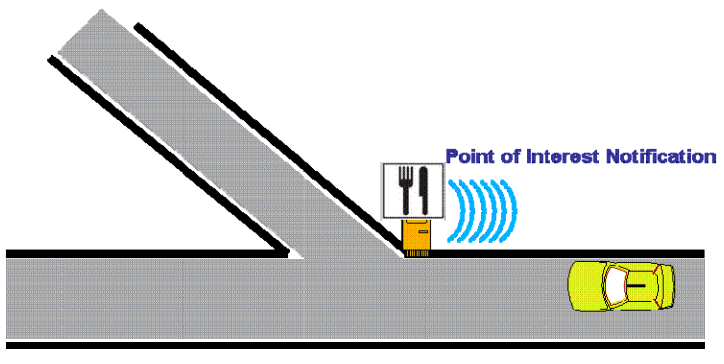
\includegraphics[width=0.99\textwidth]{content/images/06_use_cases/poin.png}
\caption{Point of Interest Notification Use Case}
\label{fig:poin}
\end{figure}

\subsubsection{Remote Diagnostics}
Der Remote Diagnostics Anwendungsfall beschreibt ein Szenario zum Warten des Autos ohne dafür in eine Werkstatt fahren zu müssen. Dadurch können Informationen über das Fahrzeug abgerufen werden und mit Hilfe der Problembeschreibung des Fahrers kann schnell festgestellt werden um was es sich handelt. Die Daten über Werkstattbesuche und was an dem Auto angefallen ist soll alles in eine Datenbank geschrieben werden sodass die Werkstatt die das Fahrzeug wartet immer weiss was gemacht worden ist. So wird die Zeit die für die Wartung eines Fahrzeuges reduziert und damit auch die Länge des Besuches in der Werkstatt für den Kunden. Um die Software eines Autos aktuell zu halten wird überhaupt kein Werkstattbesuch mehr benötigt, da das update direkt beispielsweise über das Internet geladen werden kann.
\begin{figure}[htbp]
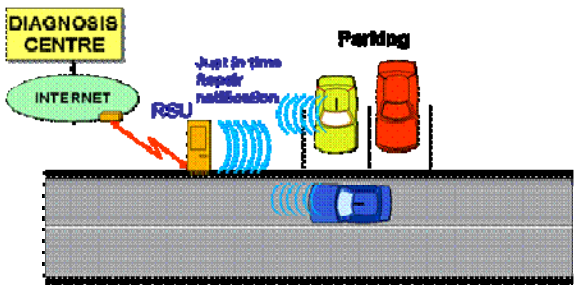
\includegraphics[width=0.99\textwidth]{content/images/06_use_cases/rds.png}
\caption{Remote Diagnostics}
\label{fig:redia}
\end{figure}
